\documentclass[xcolor=dvipsname,t]{beamer} 

\usepackage{listings} 
\usepackage{color} 
\usepackage{xcolor}  
\usepackage{microtype} 
\usepackage{helvet} 
\usepackage{inconsolata} 
\usepackage[framemethod=TikZ]{mdframed} 
\usepackage{graphicx} 
\usepackage{alltt}
\usepackage{sverb} 
\usepackage{verbatim} 

\title{A Comparison of \\Computer Security Evaluation Criteria} 
\subtitle{433-463 Software Engineering Thesis} 
\author{Michael Papasimeon} 
\date{October 1997} 


\begin{document}

\maketitle

\begin{frame}{Outline}
    \begin{itemize}
        \item Computer Security and Evaluation Criteria
        \item Comparison Characteristics
        \item The Choice of Evaluation Criteria
        \item Description of TCSEC
        \item Description of ITSEC
        \item Description of CTCPEC
        \item Conclusions
    \end{itemize}
\end{frame}

\begin{frame} {Computer Security}
    \begin{itemize}
        \item Security Functionality
        \item Security Assurance
    \end{itemize}
    \begin{center}
        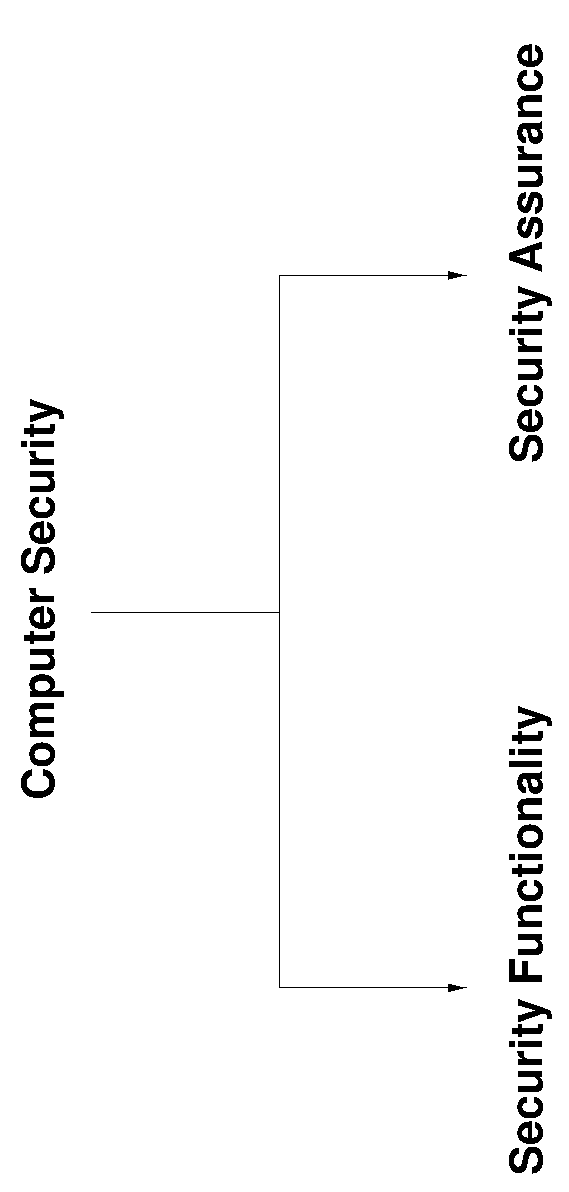
\includegraphics[angle=-90, width=7cm]{tree.eps}
    \end{center}
\end{frame}

\begin{frame} {Security Functionality}
    Examples include security features such as:
    \begin{itemize}
        \item Identification
        \item Authentication
        \item Discretionary and Mandatory Access Control
        \item Auditing
        \item Encryption
    \end{itemize}
\end{frame}

\begin{frame} {Security Assurance}
    Typically involves the use of strict Software Engineering practices
    with an emphasis on assuring functionality.
    \begin{itemize}
        \item Security Policy and Security Policy Model Specification
        \item System Design
        \item Implementation
        \item Security Testing
        \item Security Documentation
        \item Configuration Management
        \item Verification and Validation of the development process
    \end{itemize}
\end{frame}

\begin{frame} {What are Computer Security Evaluation Criteria?}
    \begin{itemize}
        \item General security standards
        \item Provide a set of criteria or requirements relating
              to security functionality and assurance
        \item Criteria are usually divided into ``Levels of Trust''
              or ratings
        \item Computer systems are evaluated against a set of
              criteria and are given the rating or ''Level of Trust''
              of which they satisfy they have satisfied the requirements.
        \item A metric for measuring the level of security provided
              and confidence in that security provided by a system.
    \end{itemize}
\end{frame}

\begin{frame} {Typical Evaluation Process (1)} 
    \vspace{1cm}
    \begin{center}
        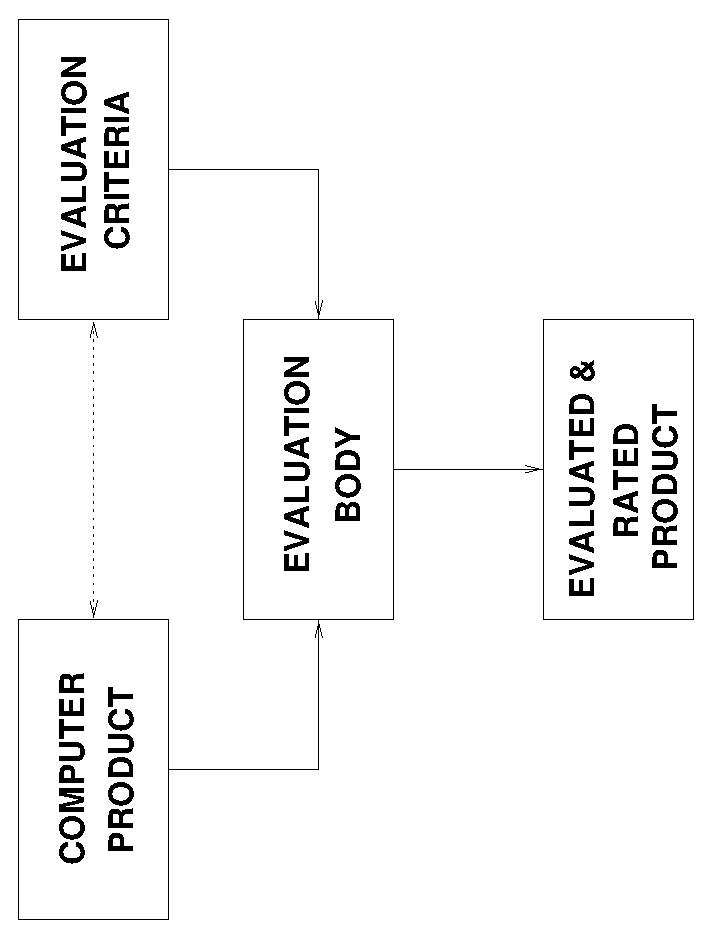
\includegraphics[angle=-90, width=7cm]{process.eps}
    \end{center}
\end{frame}

\begin{frame} {Typical Evaluation Process (2)}
    \vspace{1cm}
    \begin{center}
        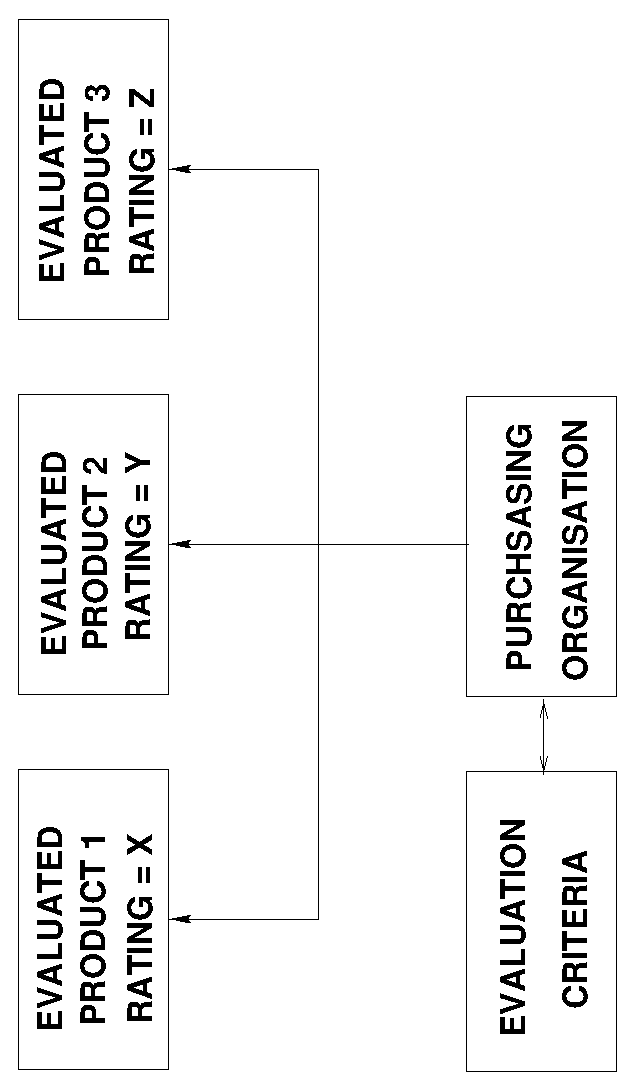
\includegraphics[angle=-90, width=7.5cm]{customer.eps}
    \end{center}
\end{frame}

\begin{frame} {Comparison Characteristics}
    \begin{enumerate}
        \item Organisation
            \begin{itemize}
                \item Structure, Scope, Approach
                \item Levels of Trust
            \end{itemize}
        \item Security Functionality
            \begin{itemize}
                \item Accountability -- Identification and Authentication
                \item Access Control
                \item Audit
            \end{itemize}
        \item Security Assurance
            \begin{itemize}
                \item Security Policy
                \item System Design
                \item Implementation
                \item Security Testing
                \item Security Documentation
                \item Configuration Management
            \end{itemize}
    \end{enumerate}
\end{frame}

\begin{frame} {Security Evaluation Criteria (1)}
    \begin{itemize}
        \item United States
            \begin{itemize}
                \item Trusted Computer System Evaluation Criteria (TCSEC)\\
                      Also known as ``Orange Book''
                \item Federal Criteria
            \end{itemize}
        \item Canada
            \begin{itemize}
               \item Canadian Trusted Computer Product Evaluation Criteria (CTCPEC) 
            \end{itemize}
    \end{itemize}
\end{frame}

\begin{frame} {Security Evaluation Criteria (2)}
    \begin{itemize}
        \item Europe
        \begin{itemize}
            \item UK Systems Security Level
            \item UK Commercial Computer Security Centre Evaluation
                  Levels Manual
            \item German Criteria for the Evaluation of Trustworthiness
                  of Information Technology Systems
            \item French ``Blue-White-Red'' Book
            \item Information Technology Security Evaluation Criteria (ITSEC)
                  [UK, France, Germany, the Netherlands]
        \end{itemize}
        \item International
        \begin{itemize}
            \item Common Criteria (CC)
        \end{itemize}
    \end{itemize}
\end{frame}

\begin{frame} {Security Evaluation Criteria Selected for Comparison}
    The most influential and widely used evaluation criteria were selected
    for the comparison.
    \begin{itemize}
        \item Trusted Computer System Evaluation Criteria (TCSEC) [Orange Book]
        \item Information Technology Security Evaluation Criteria (ITSEC)
        \item Canadian Trusted Computer Product Evaluation Criteria (CTCPEC)
    \end{itemize}
\end{frame}

\begin{frame} {TCSEC (Orange Book)}
    \begin{itemize}
        \item Classes contain both security functionality
              and security assurance requirements
        \item Scope is very high level
        \item Interpretation documents (The Rainbow Series)
              required for more specific cases. (eg: The Red Book
              is the Trusted Network Interpretation of the Orange Book).
    \end{itemize}
\end{frame}

\begin{frame} {TCSEC -- Evaluation Criteria Classes}
    \begin{itemize}
        \item D -- Minimal Protection
        \item C1 -- Discretionary Security Protection
        \item C2 -- Controlled Access Protection
        \item B1 -- Labelled Security Protection
        \item B2 -- Structured Protection
        \item B3 -- Security Domains
        \item A1 -- Verified Design
    \end{itemize}
\end{frame}

\begin{frame} {TCSEC Class Requirements} 
    \begin{enumerate}
        \item Security Policy
        \item Accountability
        \item Assurance
        \item Documentation
    \end{enumerate}
\end{frame}

\begin{frame} {CTCPEC}
    \begin{itemize}
        \item Divides criteria into functionality criteria
              and asssurance criteria
        \item Does not require separate interpretation documents 
              as it has more specific criteria
    \end{itemize}
\end{frame}

\begin{frame} {CTCPEC Assurance Levels}
    \begin{itemize}
        \item Assurance Level T0
        \item Assurance Level T1
        \item Assurance Level T2
        \item Assurance Level T3
        \item Assurance Level T4
        \item Assurance Level T5
        \item Assurance Level T6
        \item Assurance Level T7
    \end{itemize}
\end{frame}

\begin{frame} {CTCPEC Assurance Levels -- Areas of Evaluation}
    \begin{itemize}
        \item Architecture
        \item Development Environment
        \item Development Evidence
        \item Operational Environment
        \item Security Documentation
        \item Security Testing
    \end{itemize}
\end{frame}

\begin{frame} {CTCPEC Functionality Criteria}
    \begin{enumerate}
        \item Confidentiality Criteria
        \item Integrity Criteria
        \item Availability Criteria
        \item Accountability Criteria
    \end{enumerate}
\end{frame}

\begin{frame} {ITSEC}
    \begin{itemize}
        \item Separation of assurance and functionality criteria
        \item Security functionality classes are not provided
        \item Only examples functionality classes and guidelines
              are provided
        \item Does not depend on external interpretation documents
    \end{itemize}
\end{frame}

\begin{frame} {ITSEC Assurance Levels}
    \begin{itemize}
        \item Assurance Level E0
        \item Assurance Level E1
        \item Assurance Level E2
        \item Assurance Level E3
        \item Assurance Level E4
        \item Assurance Level E5
        \item Assurance Level E6
    \end{itemize}
\end{frame}

\begin{frame} {ITSEC Assurance Levels -- Areas of Evaluation}
    \begin{enumerate}
        \item Development Process
            \begin{itemize}
                \item Requirements Specification
                \item Architectural Design
                \item Detailed Design
                \item Implementation
            \end{itemize}
        \item Development Environment
            \begin{itemize}
                \item Configuaration Control
                \item Programming Languages and Compilers
                \item Developer's Security
            \end{itemize}
        \item Operational Documentation
            \begin{itemize}
                \item User Documentation
                \item Administrator Documentation
            \end{itemize}
        \item Operational Environment
            \begin{itemize}
                \item Delivery and Configuration
                \item Start-up and Operation
            \end{itemize}
    \end{enumerate}
\end{frame}

\begin{frame} {ITSEC Example Functionality Classes}
    \begin{itemize}
        \item Functionality Class F-C1
        \item Functionality Class F-C2
        \item Functionality Class F-B1
        \item Functionality Class F-B2
        \item Functionality Class F-B3
        \item Functionality Class F-IN
        \item Functionality Class F-AV
        \item Functionality Class F-DI
        \item Functionality Class F-DC
        \item Functionality Class F-DX
    \end{itemize}
\end{frame}

\begin{frame} {ITSEC Functionality Class Specification Guidelines}
    \begin{itemize}
        \item Identification and Authentication
        \item Access Control
        \item Audit
        \item Object Reuse
        \item Accuracy
        \item Reliability of Service
        \item Data Exchange
    \end{itemize}
\end{frame}

\begin{frame} {Consequences}
\end{frame}

\begin{frame} {Summary}
\end{frame}

\end{document}

